\documentclass[11pt, letterpaper]{article}
\usepackage[utf8]{inputenc}
\usepackage[letterpaper, margin=0.5in]{geometry}
\usepackage{amsmath}
\usepackage{amssymb}
\usepackage{amsthm}
\usepackage{graphicx}
\usepackage{listings}
\usepackage[font=scriptsize]{caption}
\usepackage{subcaption}
\usepackage{xcolor}

\definecolor{codegreen}{rgb}{0,0.6,0}
\definecolor{codegray}{rgb}{0.5,0.5,0.5}
\definecolor{codepurple}{rgb}{0.58,0,0.82}
\definecolor{backcolour}{rgb}{0.95,0.95,0.92}

\lstdefinestyle{mystyle}{
    backgroundcolor=\color{backcolour},   
    commentstyle=\color{codegreen},
    keywordstyle=\color{magenta},
    numberstyle=\tiny\color{codegray},
    stringstyle=\color{codepurple},
    basicstyle=\ttfamily\footnotesize,
    breakatwhitespace=false,
    texcl=true,
    mathescape=true,
    breaklines=true,                 
    captionpos=b,                    
    keepspaces=true,                 
    numbers=left,                    
    numbersep=5pt,                  
    showspaces=false,                
    showstringspaces=false,
    showtabs=false,                  
    tabsize=2
}

\lstset{style=mystyle}
\graphicspath{ {.} }
\captionsetup{justification=raggedright, singlelinecheck=false}

\author{Ryan Tang}
\title{STA 602 HW 11}
\date{November 18th 2022}

\begin{document}
\maketitle

\section{Exercise 9.1}
\paragraph{(a) Analysis}
We have the following graphical model, one for each swimmer $k \in \{1, \dots, K=4\}$. For each swimmer, we have worth of 6 weeks of data points that records their swim time for a 50 yards run, $i \in \{1, \dots, N=6\}$. Here we like to fit a linear regression for each swimmer; thus, in total of 4 linear regression, each with its respective priors.
\begin{figure*}[!h]
  \centering
  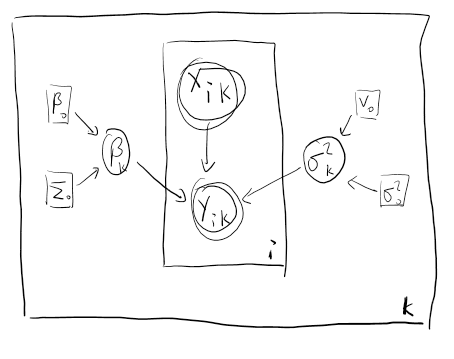
\includegraphics[width=0.4\textwidth]{1.2.graph.png}
  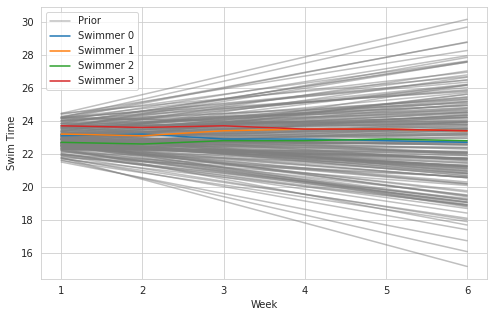
\includegraphics[width=0.45\textwidth]{1.1.png}
  % \captionsetup{justification=centering}
  \caption{(Left) Typical Bayesian Linear Regression Graphical Model. (Right) Prior Believe Check. Each grey line is a sampled prediction using just the priors.}
\end{figure*}

We are also given some knowledge on typical competitive times for the age group range from 22 to 24 seconds. We will use this to construct out priors accordingly, and the following is the full spec of the model. Some notations, $X_{k} \in \mathbf{R}^{N\times p}$, $\bold{y}_k \in \mathbf{R}^N$, and $\beta_k \in \mathbf{R}^p$, where $p = 2$ in our case, one for the intercept, and one for the weeks.
\begin{align*}
    \bold{y}_{ik} &\mathop{\thicksim}^{iid} \mathcal{N}(X_k \beta_k, \sigma_k^2 \mathbf{I}_n) \\
    \beta_k &\thicksim \mathcal{N}(\beta_o, \Sigma_o) \\
    1/\sigma^2_k = \gamma_k &\thicksim \text{Gamma}(\frac{\nu_o}{2}, \frac{\nu_o\sigma^2_o}{2})
\end{align*}
Here we specified $\beta_o = (23, 0)^{\intercal}$, $\Sigma_o = \begin{bmatrix}0.2 & 0 \\ 0 & 0.2\end{bmatrix}$, $\nu_0 = 1$, $\sigma^2_o = 1$, and the resulting prior believes is also plotted in Figure 1, right plot.


\section{Exercise 9.2}
\section{Exercise 9.3}


\end{document}